\section{\label{qleet-sec:abstract}Abstract}

We present qLEET, an open-source Python package for studying parameterized quantum circuits (PQCs), which are widely used in various variational quantum algorithms (VQAs) and quantum machine learning (QML) algorithms. qLEET enables computation of properties such as expressibility and entangling power of a PQC by studying its entanglement spectrum and the distribution of parameterized states produced by it. Furthermore, it allows users to visualize the training trajectories of PQCs along with high-dimensional loss landscapes generated by them for different objective functions. It supports quantum circuits and noise models built using popular quantum computing libraries such as Qiskit, Cirq, and Pyquil. In our work, we demonstrate how qLEET provides opportunities to design and improve hybrid quantum-classical algorithms by utilizing intuitive insights from the ansatz capability and structure of the loss landscape.

\section{\label{qleet-sec:intro}Introduction}

Parameterized quantum circuits (PQCs) are one of the fundamental components of variational quantum algorithms (VQAs). They are responsible for evolving the qubits system to a state dependent on the series of parameters ($\vec{\theta}$) provided by a classical processor and the objective function where the initial state of the qubit system might be the ground state $\ket{0\ldots0}$, or some other state $\ket{\psi_0}$ of a particular form. The PQC ($U(\vec{\theta})$) is also popularly referred to as ansatz, as we have already seen in the previous two chapters. Their structure dramatically affects the performance of VQAs as they influence both (i) convergence speed, i.e., the number of quantum-classical feedback iterations, and (ii) closeness of the final state ($\ket{\psi({\vec{\theta}})}$) to a state that optimally solves the problem ($\ket{\psi({\vec{\theta}^*})}$), i.e., the overlap or the fidelity ($\mathcal{F} = |\langle\psi({\vec{\theta})} | \psi({\vec{\theta}^*})\rangle|^{2}$) between the final state and the target state. 

Therefore, it becomes imperative to be able to design PQCs for a given problem. However, this is not straightforward because their design depends not only on the problem itself but also on the quantum hardware that executes them. After all, some essential properties like depth of circuit post compilation depend on the hardware's topology and the supported basis gates. Nevertheless, based on this, there exist three main classes of ansätze: (i) problem-inspired ansatz, where the evolutions of generators derived from properties of the given system are used to construct the PQCs, (ii) hardware-efficient ansatz, where a minimal set of quantum gates native to a given device are used to construct the PQCs, (iii) adaptive ansatz, which is midway between the former two ansätze. Using these three classes, one can come up with numerous ansatz designs for any given problem, but to finally choose one, we need to compare them.

The primary motivation behind the development of qLEET\footnote{\href{https://github.com/QLemma/qleet}{https://github.com/QLemma/qleet}} \cite{qleet-zenodo} stems from this need to have a framework for analyzing the capabilities of parameterized quantum circuits. It does so by allowing users to study various properties related to the behavior of PQCs and assess their trainability. In particular, it will enable visualization of the loss landscape of a PQC for a given objective function and its training trajectory in the parameter space. Furthermore, it allows calculation of some essential properties of PQCs, such as their expressibility and entangling capabilities \cite{expressibility-entanglability-guzik}. It is integrable with other popular libraries such as Qiskit \cite{comp_qiskit}, Cirq \cite{comp_cirq}, or PyQuil \cite{ccquad_Pyquil} and also supports instruction-set languages like OPENQasm \cite{2021arXiv210414722C} and Quil \cite{ccquad_Pyquil}.

\begin{figure*}[!htp]
    \centering
    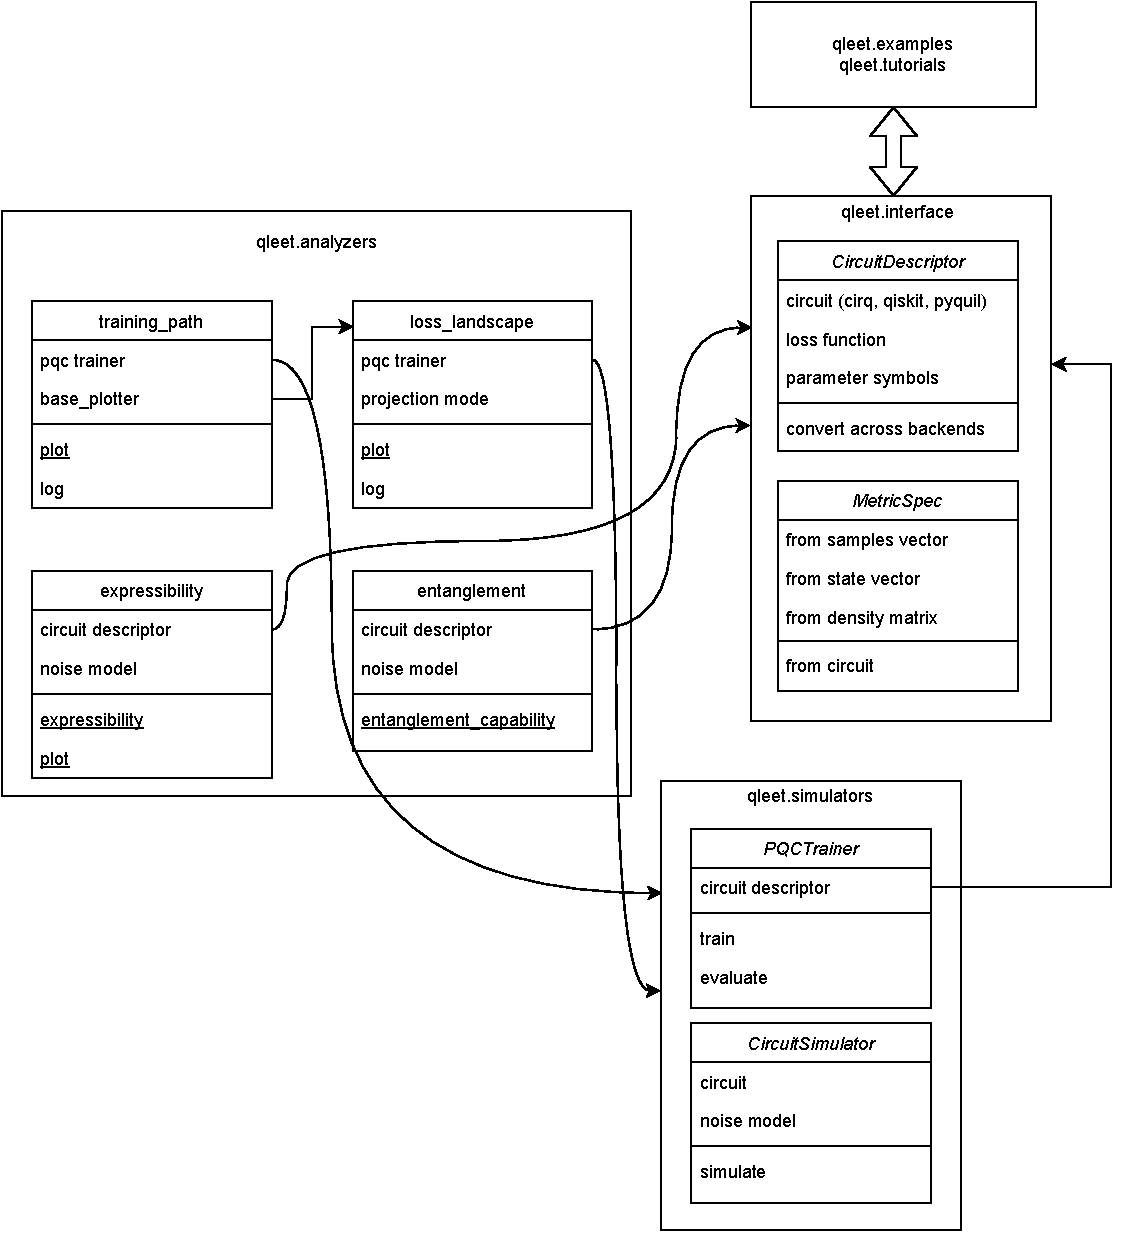
\includegraphics[width=0.5\linewidth]{figures/qleet/qleet-architecture.pdf}
    \caption{Architecture stack for qLEET}
    \label{qleet-fig:qleet-architecture}
\end{figure*}

\section{Overview}

We implement qLEET by following a modular approach where similar functionalities are grouped under one single module that can interact with one another, as shown in Fig. \ref{qleet-fig:qleet-architecture}. In total, there exist the following three modules:
\begin{enumerate}
	\item \textbf{Interface module}: This allows building either PQC or the workflow of the variational computation by also specifying a set of parameters, objective or cost function, and metrics based on the final state to which the circuit evolves. It also provides a circuit wrapper called \texttt{CircuitDescriptor} that makes the computation hardware agnostic. 
	\item \textbf{Simulators module}: This module helps train in setting up the training routine (\texttt{PQCTrainer}) for the variational computations and simulations routine (\texttt{CircuitSimulator}) for standalone PQCs with or without noise depending upon whether the user provides a noise model or not.
	\item \textbf{Analyzers module}: This module takes in a \texttt{CircuitDescriptor} or \texttt{CircuitSimulator} object to compute various properties such as loss landscape or training trajectory in the case of a variational computation and expressibility or entangling capacity value for standalone PQCs.
\end{enumerate}

In addition to these, we provide add-ons in the form of tutorials and predefined examples. Furthermore, we list below the theory for a range of features that are supported by qLEET.

\begin{figure*}[!tp]
    \centering
    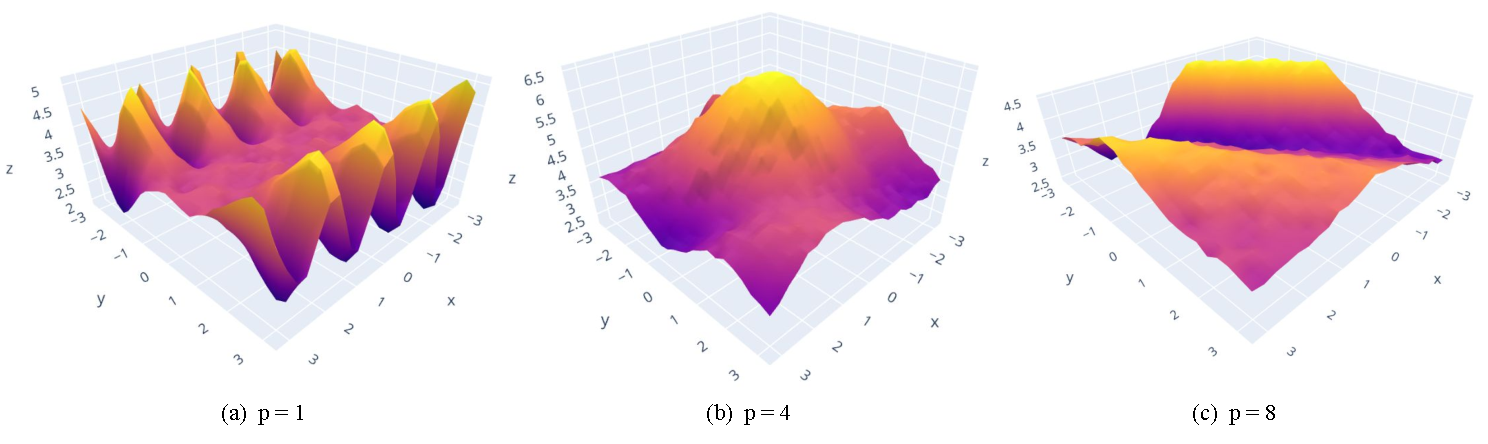
\includegraphics[width=\linewidth]{figures/qleet/loss-landscape.pdf}
    \caption[Loss landscapes for QAOA]{Loss landscapes for solving Max-Cut problem for an Erdos-Renyi graph with $12$ nodes and $0.5$ edge probability, using QAOA for different values of $p$.}
    \label{fig:qleet-loss}
\end{figure*}

\section{Trainability of PQCs}

Let us consider a PQC $\hat{U}(\vec{\theta})$ and an objective function $\mathcal{C}$. The process of training of $U(\vec{\theta})$ with respect to $\mathcal{C}$ is defined as:
\begin{equation}
	\mathcal{C} = \min \text{Tr}[O\rho(\vec{\theta}_t)]
\end{equation}
\begin{equation}
     \vec{\theta}_{t+1} = \vec{\theta}_t - \gamma\nabla_{\vec{\theta}}\ \mathcal{C}
\end{equation}

Here, $\rho(\vec{\theta})$ is an arbitrary quantum state produced by the PQC, and $\hat{O}$ is a Pauli observable. This Pauli observable can either be a physical Hamiltonian (as in the case of molecular VQE) or any other Hermitian observable. To assess the trainability of PQC, we would require to calculate the $\mathcal{C}$ and also the contribution of a parameter $\theta_v$ to $\nabla_{\vec{\theta}}\ \mathcal{C}$, i.e., $\partial\mathcal{C}/\partial\theta_v$. For a majority of values, these contributions will be unbiased, non-vanishing, and non-exploding, the PQCs can be trained successfully for the given $\mathcal{C}$. These could be better understood by visualizing the loss landscape and training path.

\subsection{Loss Landscape}

Loss landscape is a visual representation of the loss value of different areas of our parameter space, of how different parameter vectors result in states with different values of the objective . We perform this analysis typically around the point of convergence $\theta^*$ to visualize the smoothness of loss surface and identify features like local minima, barren plateaus, ridges and valleys, etc. \cite{loss-landscapes}

To plot the loss landscape, we compute the loss function value for all the parameters in the orthonormalized 2-D subspace $S$ with basis vectors $\theta_i$ sampled from the whole parameter space as detailed in equation \ref{qleet-eqn:loss-landscape-plot}. Based on how this sampling is performed, we can gather different information about the landscape. For example, suppose we use a principal component analysis (PCA) over the set of parameters at each training step. In that case, we get the vectors, i.e., the directions in space for which major movements occurred for our PQC during training. Similarly, other methods for obtaining subspace could be used, such as doing random sampling of basis vectors or t-SNE (t-Distributed Stochastic Neighbor Embedding) of the parameter vectors encountered in the training trajectory. We gain some crucial insights from the loss landscape, such as the roughness, flatness, and the presence of repeating patterns, which could help one adapt our training strategy by tweaking the optimization routine, evaluation metric, etc. 

\begin{equation}\label{qleet-eqn:loss-landscape-plot}
    \begin{split}
        f(\alpha_i) 
        &= \mathcal{C}_{\text{PQC}}(\theta^* + \sum_i \alpha_i \theta_i) \\ 
        &= \sum_{O} \text{Tr}\Bigg[O\rho \bigg(\vec{\theta^* + \sum_i \alpha_i \theta_i} \bigg) \Bigg]
    \end{split}
\end{equation}

\begin{figure}[!tp]
    \centering
    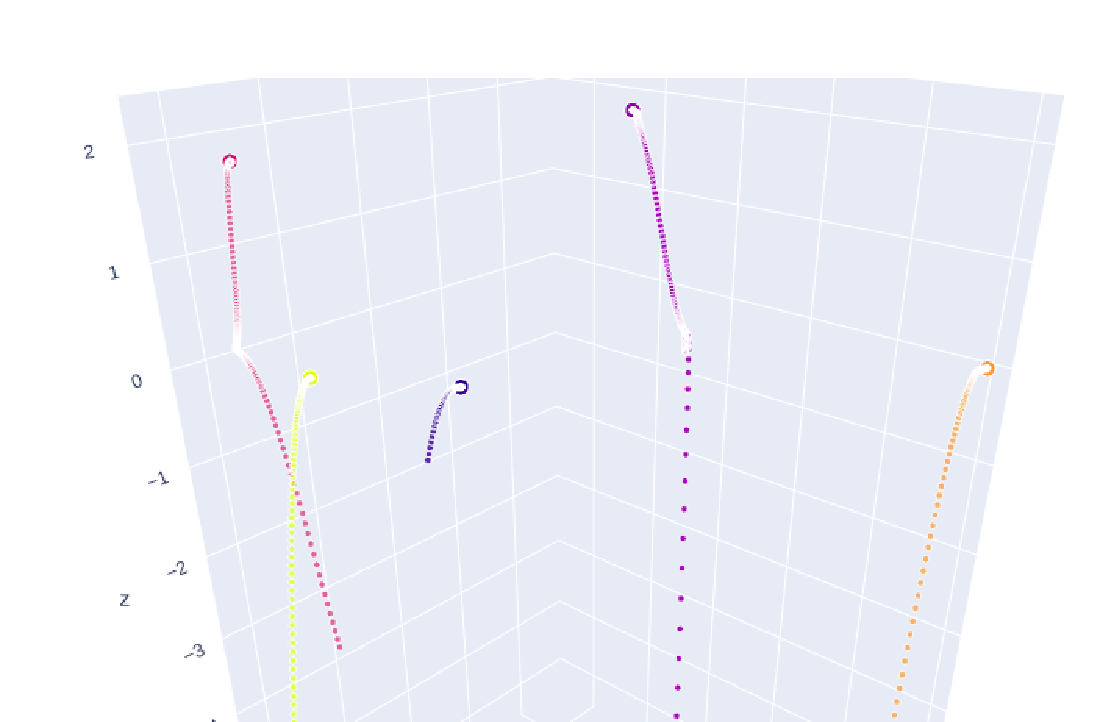
\includegraphics[width=\linewidth]{figures/qleet/training-trajectories.pdf}
    \caption[Parameters in from several Training Trajectories]{This shows a 2-D projection of the parameter vectors plotted on the X-Y axes for 5 different re-initializations, each shown using a different color. These are collected over the entire optimization run and the final value of each run is plotted with a larger blob, visible at the top of each trajectory. The z-axis shows the loss value at that parameter vector. In this plot, it is visible that the trajectories do not mix and instead ascend up their own local optima, which indicates that sufficient exploration of the loss landscape was not performed and the optimization was very much local in nature and vary over different runs.}
    \label{qleet-fig:training-trajectories}
\end{figure}

\subsection{Training Trajectory}

In addition to the loss landscape, it is also essential to visualize the training paths for PQC. Plotting these training trajectories over several re-initializations helps us learn about convergence properties of the parametrized quantum circuits and their optimization schedules. We plot the entire set of parameter vectors over all the re-initializations collected from each timestep of the training process $\theta_{k}^{t}$. Similar to the loss landscapes visualization, we project these parameter vectors down to a 2-dimentional subspace which can be chosen randomly, via PCA of encountered parameter vectors, or t-SNE of the same. The 2-D projections of the parameter trajectories can also be plotted on the loss surface, with the loss values on the 3rd axis. \cite{training-trajectories}

\begin{figure*}[!tp]
    \centering
    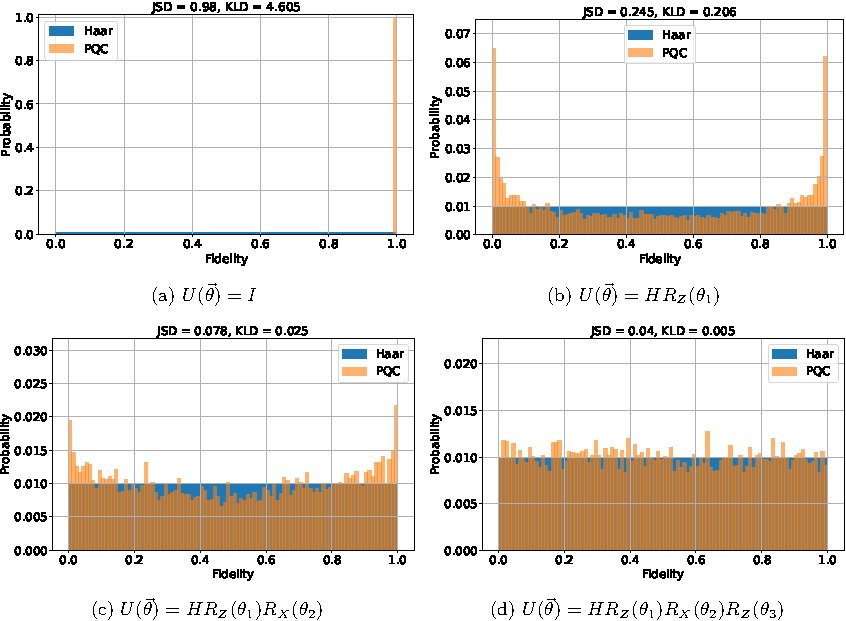
\includegraphics[width=\textwidth]{figures/qleet/expressibility.pdf}
    \caption[Quantifying expressibility for single-qubit circuits]{Quantifying expressibility for single-qubit circuits. For each of the four circuits show here, 1000 sample pairs of circuit parameter vectors were uniformly drawn, corresponding to 2000 parameterized states. Histograms of estimated fidelities (orange) are shown, overlaid with fidelities of the Haar-distributed ensemble (blue), with the computed Kullback-Leibler (KL) and Jensen-Shannon Distance (JS) divergences reported above the histograms.}
    \label{qleet-fig:expressibility}
\end{figure*}

\subsection{Expressibility}

Sampling states $\ket{\psi(\vec{\theta})}$ from a PQC, $\hat{U}(\vec{\theta})$, for a randomly sampled parameter vector $\vec{\theta}$ generates a distribution of states. The deviation of this distribution from the Haar measure is defined as \textit{Expressibility}, where the Haar measure samples the full Hilbert space uniformly.

\begin{equation}\label{qleet-qleet:eq3}
A^{(t)}=\left\Vert \int_\text{Haar}(\ket{\psi}\bra{\psi})^{\otimes t} \text{d}\psi-\int_{\vec{\theta}}(\ket{\psi(\vec{\theta})}(\bra{\psi(\vec{\theta})})^{\otimes t} \text{d}\psi(\vec{\theta}) \right\Vert_\text{HS}^2\,
\end{equation}

where $\int_\text{Haar}\text{d}\psi$ denotes the integration over a state $\ket{\psi}$ distributed according to the Haar measure and $\left\Vert A \right\Vert_\text{HS}^2=\text{Tr}(A^\dagger A)$ the Hilbert-Schmidt norm. As shown in \cite{expressibility-entanglability-guzik}, we can compute the quantity in Eq. \ref{qleet-qleet:eq3} as the divergence between the resulting distribution of state fidelities generated by the sampled ensemble of parameterized states to that of the ensemble of Haar random states.

\begin{equation}
    \text{Expr} = D(\hat{P}_{PQC}(F; \theta) | P_{Haar}(F))
\end{equation}

An ansatz circuit $U$ with a small \textit{Expr} value is more expressive because it would mean that the states generated by it match the Haar measure more closely. This is represented in Fig. \ref{qleet-fig:expressibility}, where we see the fidelity distribution of PQC and Haar measure increases as the single-qubit circuit is made more expressive by adding Pauli rotation gates. In general, when we train a PQC to represent a particular unknown target state, it is more likely for a highly expressive PQC to be able to represent the target state. Hence, Expressibility is a crucial measure to compare the effectiveness of a pair of PQCs. 

\subsection{Entangling Capability}

Another important quantifier for PQC is its power to create entangled states. In general, people use different kinds of entanglement measures to capture different properties of multipartite entanglement present in the system. In \cite{expressibility-entanglability-guzik}, Meyer-Wallach $Q$ measure \cite{doi:10.1063/1.1497700} has been proposed to estimate the number of entangled states can be produced by a PQC, by measuring the average entanglement between individual qubits and the rest. The entangling capability of a PQC is then defined as the average, $Q$, of states randomly sampled from the circuit.

\begin{equation}
	Q = \frac{2}{|\vec{\theta}|}\sum_{\theta_{i}\in \vec{\theta}}\Bigg(1-\frac{1}{n}\sum_{k=1}^{n}\text{Tr}(\rho_{k}^{2}(\theta_{i}))\Bigg)
\end{equation}

where $\rho_k$ is the density matrix of the $k$-th qubit. Similarly, there is another measure called Scott Measure \cite{10.1007/s11128-007-0052-7}, which is a generalized version of the Meyer-Wallach measure. It gives $m$ entanglement measures, each of which will measure the average entanglement between blocks of $m$ qubits and the rest of the system. As $m$ increases, $Q_m$ becomes more sensitive to correlations of an increasingly global nature. The entangling capability of a PQC in this case is defined by a sequence of the following $Q_m$ measures:


\begin{equation}
    \begin{split}
        Q_{m} &= \frac{2^{m}}{(2^{m}-1) |\vec{\theta}|}\sum_{\theta_i \in \vec{\theta}} \bigg(1 - \frac{m! (n-m)!)}{n!}\sum_{|S|=m} \text{Tr} (\rho_{S}^2 (\theta_i)) \bigg) \\
        m &= 1, \ldots, \lfloor n/2 \rfloor
    \end{split}
\end{equation}


\subsection{Entanglement Spectrum}

In the previous subsection, we assessed the entangling power of an ansatz using two entanglement measures. However, to fully characterize the various properties of the entanglement produced by an ansatz, one must make use of the entanglement spectrum \cite{PhysRevLett.115.267206, PRXQuantum.1.020319}, which is defined as the spectrum of eigenvalues of the entanglement Hamiltonian.

\begin{equation}
    H_{\text{ent}} = -\log (\rho_A)
\end{equation}

Here, $\rho_A = \text{Tr}_B(\rho)$ is the reduced density matrix obtained by the typical bipartition of the $N$ qubit system into subsystems $A$ and $B$. A crucial feature of $H_{\text{ent}}$ is that its eigenvalues $\xi_k$ follow the Marchenko-Pastur distribution \cite{10.1088/1751-8113/40/3/f04} for states that are sampled randomly according to Haar measure. Therefore, for a PQC, both expressibility and entangling capacity could be visualized at once by looking at the distribution of eigenvalues of $H_{\text{ent}}^{\text{PQC}}$, which is calculated from the states generated from the sampled set of parameters $\vec{\theta}$. In Fig. \ref{qleet-fig:entanglement-spectrum}, we perform the entanglement spectrum analysis on a 16 qubit PQC, which is made of $L$ layers comprising three rotation gates on each qubit and CNOT gates between adjacent qubits, i.e., $U(\vec{\theta}) = \prod_{l}^{L}\big(\prod_{i=0}^{15}R_x(\theta_i^1)R_z(\theta_i^2)R_x(\theta_i^3)\prod_{i=0}^{14}CX(i, i+1)\big)$.

\section{Challenges for Variational Quantum Computation}


\subsection{Barren Plateaus}
The Barren Plateaus (BP) phenomenon is one of the main restrictions for VQAs. For a given problem, BP will be exhibited for a cost function $\mathcal{C}(\vec{\theta})$ whose magnitude of partial derivatives will, on average, exponentially vanish. This essentially flattens the landscape, to traverse through which one would need exponentially large precision to resolve against finite sampling noise for determining a cost-minimizing direction. It was recently shown that the noise in NISQ-era hardware could induce BPs \cite{2020arXiv200714384W}. BPs are a problem of major concern because the exponential scaling in the needed precision due to BPs could erase a potential quantum advantage with a VQA, as its complexity would be comparable to the exponential scaling typically associated with classical algorithms. Therefore, to preserve the hope of using NISQ devices to achieve quantum advantage, one must attempt to build BP resilient VQAs.  

\begin{figure}[!t]
    \centering
    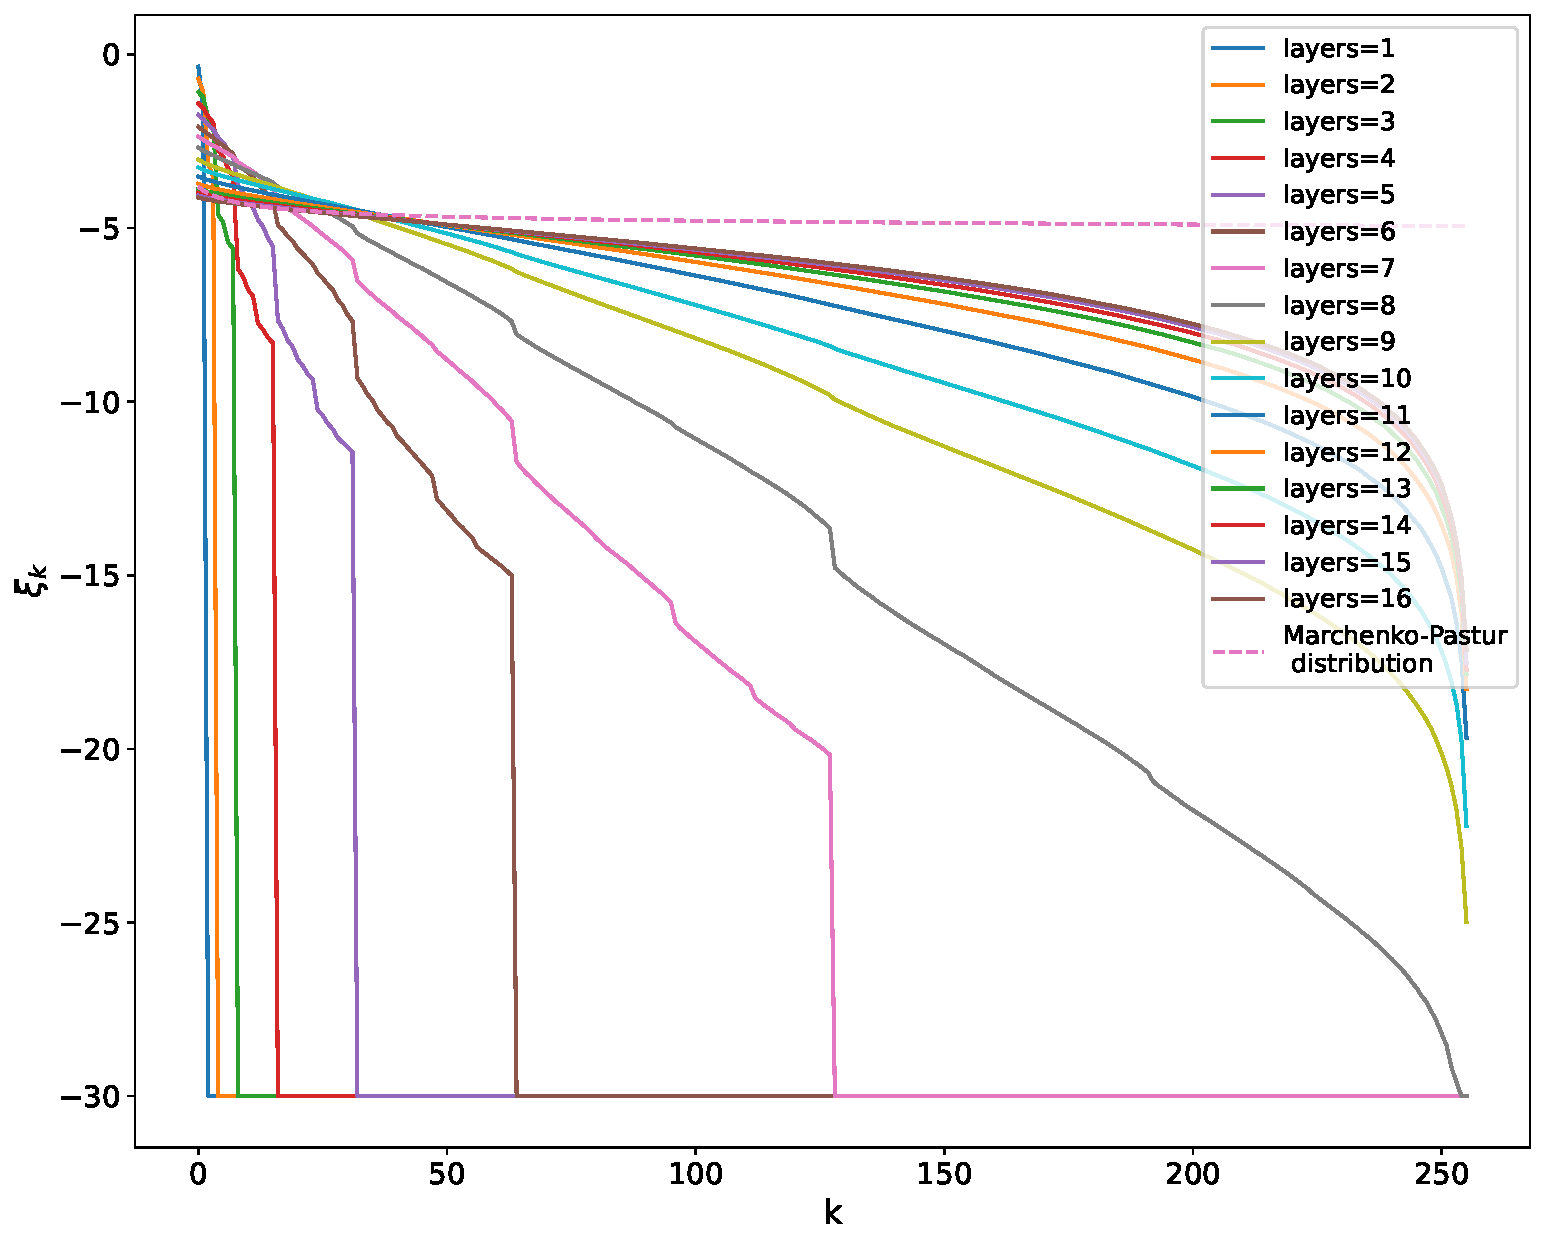
\includegraphics[width=\linewidth]{figures/qleet/entanglement-spectrum.pdf}
    \caption[Visualizing entanglement spectrum for parameterized quantum circuits]{Visualizing entanglement spectrum for a PQC $U(\vec{\theta}) = \prod_{l}^{L}\big(\prod_{i=0}^{15}R_x(\theta_i^1)R_z(\theta_i^2)R_x(\theta_i^3)\ldots\prod_{i=0}^{14}CX(i, i+1)\big)$. Here, $\xi_k$ are the eigenvalues of $H_{\text{ent}}^{U(\vec{\theta})}$ arranged in descending order and cut off at $-30$. The solid lines (blue to brown) represents the distribution $\xi_k$ for different layers $L$ and the dotted line (magenta) represents the ideal Marchenko-Pastur (MP) distribution. We see that as the number of layers is increased, the distribution of $\xi_k$ becomes more similar to MP distribution.}
    \label{qleet-fig:entanglement-spectrum}
\end{figure}



In Fig. \ref{qleet-fig:barren-plateau}, we show an example of BP phenomena while comparing global $\mathcal{C}_{Global}$ and local $\mathcal{C}_{Local}$ cost functions for learning Identity gate using a very simple ansatz: $R_X(0,\theta_1)R_X(1, \theta_2)CZ(0, 1)$. 

\begin{figure}[ht]
    \centering
    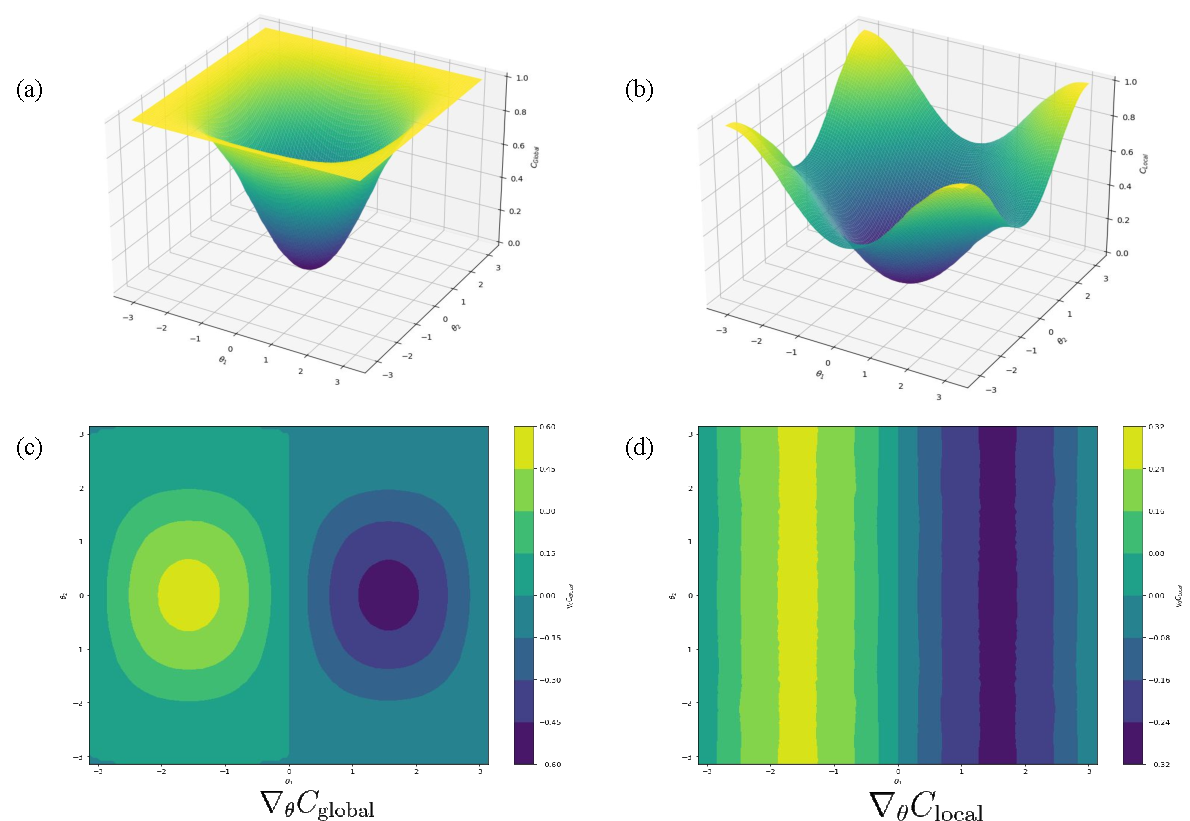
\includegraphics[width=\linewidth]{figures/qleet/barren-plateau.pdf}
    \caption[Presence of barren plateaus in parameterized quantum circuits]{Here we show the emergence of barren plateaus in the task of learning an Identity gate using the ansatz $R_X(0,\theta_1)R_X(1, \theta_2)CZ(0, 1)$ solely based on the choice of the cost function. Figures (a) and (b) represents the loss landscape for the $\mathcal{C}_{Global}$ and local $\mathcal{C}_{Local}$ cost functions, respectively. Similarly, figures (c) and (d) represents coloured heat maps for their  corresponding gradients $\nabla_{\theta}\mathcal{C}_{Global}$ and $\nabla_{\theta}\mathcal{C}_{Local}$. We see that for $\mathcal{C}_{Global}$, the gradients vanish rapidly towards the boundaries of the loss landscape.}
    \label{qleet-fig:barren-plateau}
\end{figure}

\begin{equation}
\begin{split}
    \mathcal{C}_{Global} &= \bra{\psi(\vec{\theta})} (I - \ket{0\ldots0}\bra{0\ldots0}) \ket{\psi(\vec{\theta})} \\
    &= 1 - p_{0\ldots0}
\end{split}
\end{equation}

\begin{equation}
\begin{split}
    \mathcal{C}_{Local} &= \bra{\psi(\vec{\theta})} \Bigg(I - \frac{1}{n}\sum_j \ket{0}\bra{0}_j\Bigg) \ket{\psi(\vec{\theta})} \\
    &= 1 - \frac{1}{n}\sum_j p_{0_j}
\end{split}
\end{equation}

We see how the loss landscape flattens for the $\mathcal{C}_{Global}$ and the gradients vanish exponentially as well. 

\subsection{Reachability}

Reachability quantifies whether a given PQC, $\hat{U}(\vec{\theta})$, with parameters $\vec{\theta}$ is capable of representing a parameterized quantum state $\ket{\psi(\vec{\theta})}$ that minimizes the cost function $\mathcal{C}$. Mathematically it is defined as \cite{PhysRevLett.124.090504}:

\begin{equation}
f_\text{R}=\text{min}_{\psi\in\mathcal{H}}\bra{\psi}\mathcal{C}\ket{\psi}-\text{min}_{\vec{\theta}}\bra{\psi(\vec{\theta})}\mathcal{C}\ket{\psi(\vec{\theta})},
\end{equation}

where the first term on the right side is the minimum over all states $\ket{\psi}$ of the Hilbert space, whereas the second term is the minimum over all states that can be represented by the PQC. The reachability is equal or greater than zero $f_\text{R}\ge0$, with $f_\text{R}=0$ when the PQC can generate an optimal state $\ket{\psi(\vec{\theta}^*)}$ that minimizes the objective function.

\section{Conclusion}

This chapter presents an open-source library called qLEET and demonstrates its ability to analyze various properties of parameterized quantum circuits (PQCs), such as their expressibility and entangling power. We have presented a theory of expressibility and entangling capability of a PQC based on the deviation of the distribution of parameterized states produced from the Haar measure, which samples uniformly from the entire Hilbert space. We also describe the entanglement spectrum, which allows visualizing the previous two properties at once. It also allows one to study the usage of PQCs in various variational algorithms and quantum machine learning models through its training and example modules. This involves visualizing their loss landscapes and training trajectories for different objective functions and optimizers. Finally, we discuss some critical challenges for variational quantum algorithms such as Barren Plateaus and Reachability. We conclude that qLEET will provide opportunities to design new hybrid algorithms by utilizing intuitive insights from the ansatz capability and structure of the loss landscape.
